\documentclass{jarticle}
\usepackage{SICE-SSI}
\usepackage[dvipdfmx]{graphicx}
\usepackage{amsmath}
\usepackage{url}

\begin{document}

\title{大学図書館の貸出記録による利用者の類型化}
\author{○千葉太郎\ \ 商科花子\ （千葉商科大学）}
\abstract{
  大学図書館の貸出記録から利用者の行動を類型化した．
  （ここに 3〜5 行で目的，方法，結果を書く．）
}
\keyword{クラスタリング，図書館，貸出記録}

\maketitle\thispagestyle{empty}
\pagestyle{empty}

\section{はじめに}

大学図書館の利用者は，目的によって借りる本の分野と期間が異なる\cite{tanaka2020}．
本研究では，貸出記録をクラスタリングして利用者を類型化する\footnote{データは匿名化されたものを用いた．}．

\section{方法}

\subsection{データ}

2025 年度の貸出記録 1,200 件を，分野ごとに集計して用いた\cite{suzuki2018}．記録の内訳を Table~\ref{tab:data} に示す．

\begin{table}[t]
  \centering
  \caption{Number of loans by field.}
  \label{tab:data}
  \begin{tabular}{lr}
    \hline
    Field & Loans \\
    \hline
    Literature & 480 \\
    Science & 420 \\
    Qualification & 300 \\
    \hline
  \end{tabular}
\end{table}

\subsection{分析の手法}

利用者 $i$ の特徴量を $\boldsymbol{x}_i$，クラスタ $k$ の中心を $\boldsymbol{\mu}_k$ とし，
式 \eqref{eq:kmeans} の $J$ を最小にする k-means 法\cite{macqueen1967}を用いた．
\begin{equation}
  J = \sum_{k=1}^{K} \sum_{i \in C_k} \| \boldsymbol{x}_i - \boldsymbol{\mu}_k \|^2
  \label{eq:kmeans}
\end{equation}

\section{結果}

週ごとの貸出件数を Fig.~\ref{fig:count} に示す．

\begin{figure}[t]
  \centering
  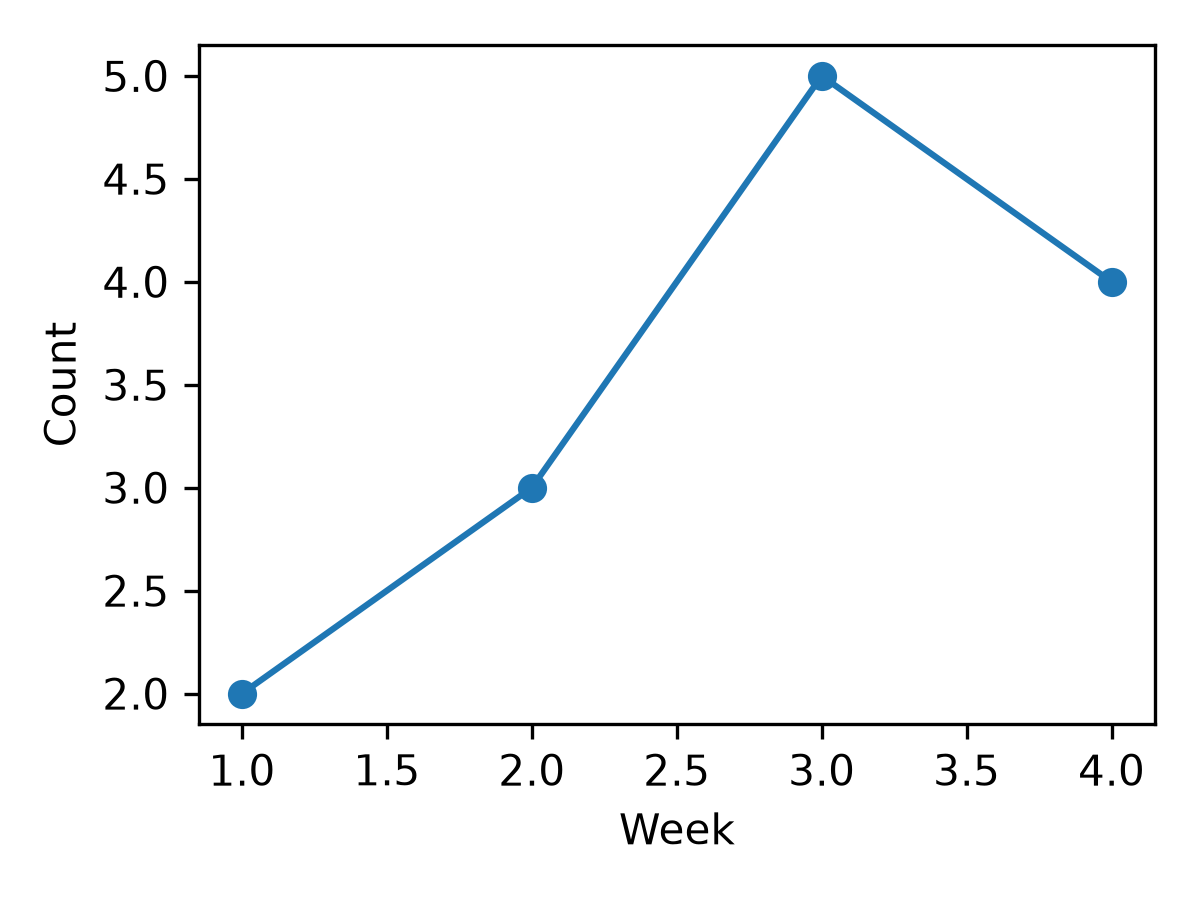
\includegraphics[width=0.9\linewidth]{figure/count.png}
  \caption{Number of loans per week.}
  \label{fig:count}
\end{figure}

\section{おわりに}

（ここに結論を書く．）

\small
\bibliographystyle{sice-ssi}
\bibliography{references}
\normalsize

\end{document}
